\subsection{Interface}
Für alle genannten Mechaniken und Informationen muss ein passendes Interface erstellt werden. Der erste Prototyp ist erkennbar in Form eines Mockups in  \autoref{image:interfaceprototype}. Das Interface wird aus einzelnen Komponenten bestehen, welche in der Grafik durch die rot markierten Bereiche erkennbar sind und in folgenden Paragraphen mit (X) referenziert werden, wobei X dem roten Bereich mit der Zahl X in \autoref{image:interfaceprototype} zugeordnet wird.

\begin{figure}
    \begin{center}
        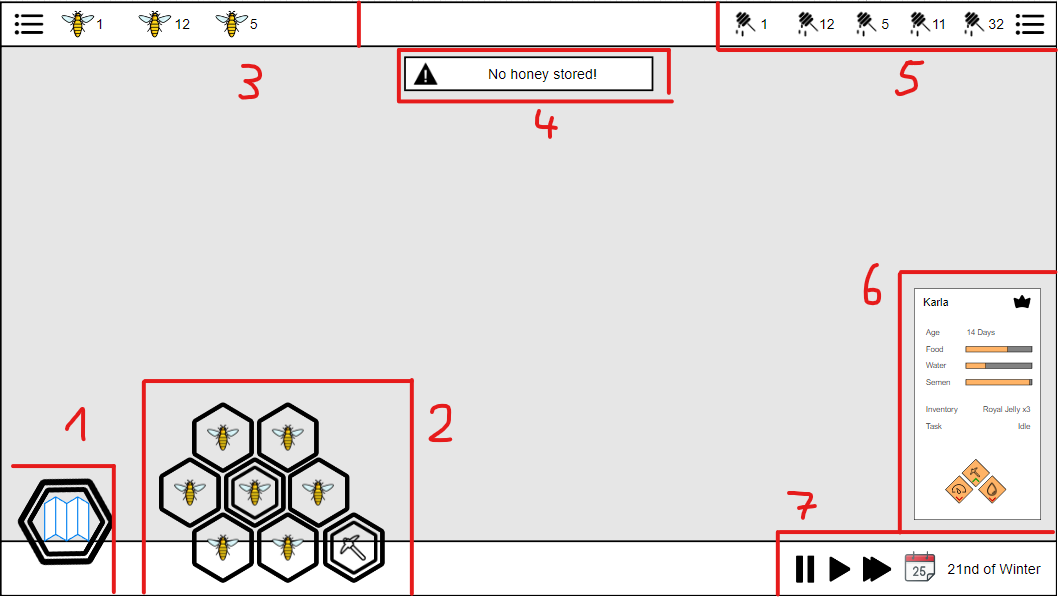
\includegraphics[width=300px]{0.bilder/interfaceprototype.png}
    \end{center}
    \caption{Erster Prototyp des Spielinterfaces} \label{image:interfaceprototype}
\end{figure}

\subsubsection{Karte wechseln}
Um zwischen der Außenwelt und dem inneren des Bienenstocks hin- und herzuwechseln gibt es den Button, welcher in Bereich (1) von \autoref{image:interfaceprototype} dargestellt wird. Befindet sich die Kamera in der Außenwelt, ist auf diesem Knopf ein Bienenstock abgebildet, befindet sich die Kamera im Bienenstock ist dort ein Baum abgebildet, welcher Symbolisch für die Außenwelt steht.

\subsubsection{Action Buttons}
Zur Steuerung der Bienen bedarf es verschiedener auswählbaren Aktionen, welche bereits zuvor erläutert wurden. Es gibt insgesamt 12 verschiedene Aktionen, welche in zwei hexagonale Menüs aufgeteilt sind, zum einen die Tätigkeiten und zum anderen die Strukturen. Diese Menu Buttons sind mit einem zweiten, inneren Hexagon markiert und in Bereich (2) auffindbar. Klickt man auf den jeweiligen Menü-Knopf öffnen sich die jeweils 6 untergeordneten Buttons. Ist währenddessen das andere Menü geöffnet, wird es geschlossen. Es kann somit maximal nur ein Menü gleichzeitig aktiv sein, aber es können beide zeitgleich geschlossen werden. Für den in der Arbeit angefertigten Prototypen werden lediglich die Aktionen \textit{Gather}, \textit{Pollinate} und \textit{Build Storage} funktional implementiert.

\subsubsection{Bee List}
Für einen besseren Überblick der Anzahl verschiedener in der Kolonie vorhandener Kasten wird eine kleine Übersicht dargestellt (3). Der Button an der linken Seite öffnet die Liste der Prioritäten, welche bereits zuvor erläutert wurde (vgl. \autoref{image:prioritylist}). Die Grafiken der jeweiligen Kaste oder des Jobs sind noch nicht unterschiedlich dargestellt.

\subsubsection{Alerts}
Damit der Spieler leichter Überblick über kritische Situationen, wie auch stattfindende Events, haben kann, wird in der Mitte des Bildschirms eine kleine Benachrichtigung visualisiert (4). Ein Alert bleibt für einen kurzen Moment und verschwindet dann wieder, der Spieler wird damit angeregt, aufmerksamer zu spielen und bedient sich der Hypothese [H8].

\subsubsection{Resource List}
Analog zu RimWorld wird dem Spieler der globale Speicherzustand aller Ressourcen angezeigt (5). Es werden also die Summen aller verschiedenen sammel- und tragbaren Ressourcen angezeigt: \textit{Nectar, Pollen, Wax, Honey} und \textit{Royal Jelly}. Der Button auf der rechten Seite ist, analog wie bei der Bee List, im Prototypen noch nicht funktional, soll aber ähnlich dazu eine Statistik offenbaren, um den Verlauf der Ressourcenstände zu visualisieren.

\subsubsection{Infofenster}
An der rechten Seite des Bildschirms ist ein Infofenster auffindbar, welches Informationen zum ausgewählten Objekt darstellt. In dem Mockup des Prototypen ist das angezeigte Infofenster jenes, welches bei Auswahl einer Biene gezeigt wird (6). Es werden unter anderem Hunger, Durst, Traits und momentane Aufgabe dargestellt.

\subsubsection{Time Control}
Ebenfalls analog zu RimWorld ist eine Zeitsteuerung implementiert, welche bereits zuvor erläutert wurde. Auf der rechten Seite dieser Steuerung wird das derzeitige Datum angezeigt in dem Format \textit{Year A, Day B of C, Dh}, wobei A das derzeitige Jahr, B der momentane Tag, C die derzeitige Jahreszeit und D die momentane Stunde ist (7).

\subsubsection{Start Screen}
Das Interface, welches dem Spieler als allererstes gezeigt wird, ist der Start Screen, welcher für den Anfang sehr simpel gehalten ist nach Hypothese [H1]. Es werden lediglich zwei Buttons zum Erstellen und Laden eines Spielstands angezeigt, ein Hintergrund des Spiels und eine Überschrift mit dem Titel des Spiels \autoref{image:startscreen}.

\begin{figure}
    \begin{center}
        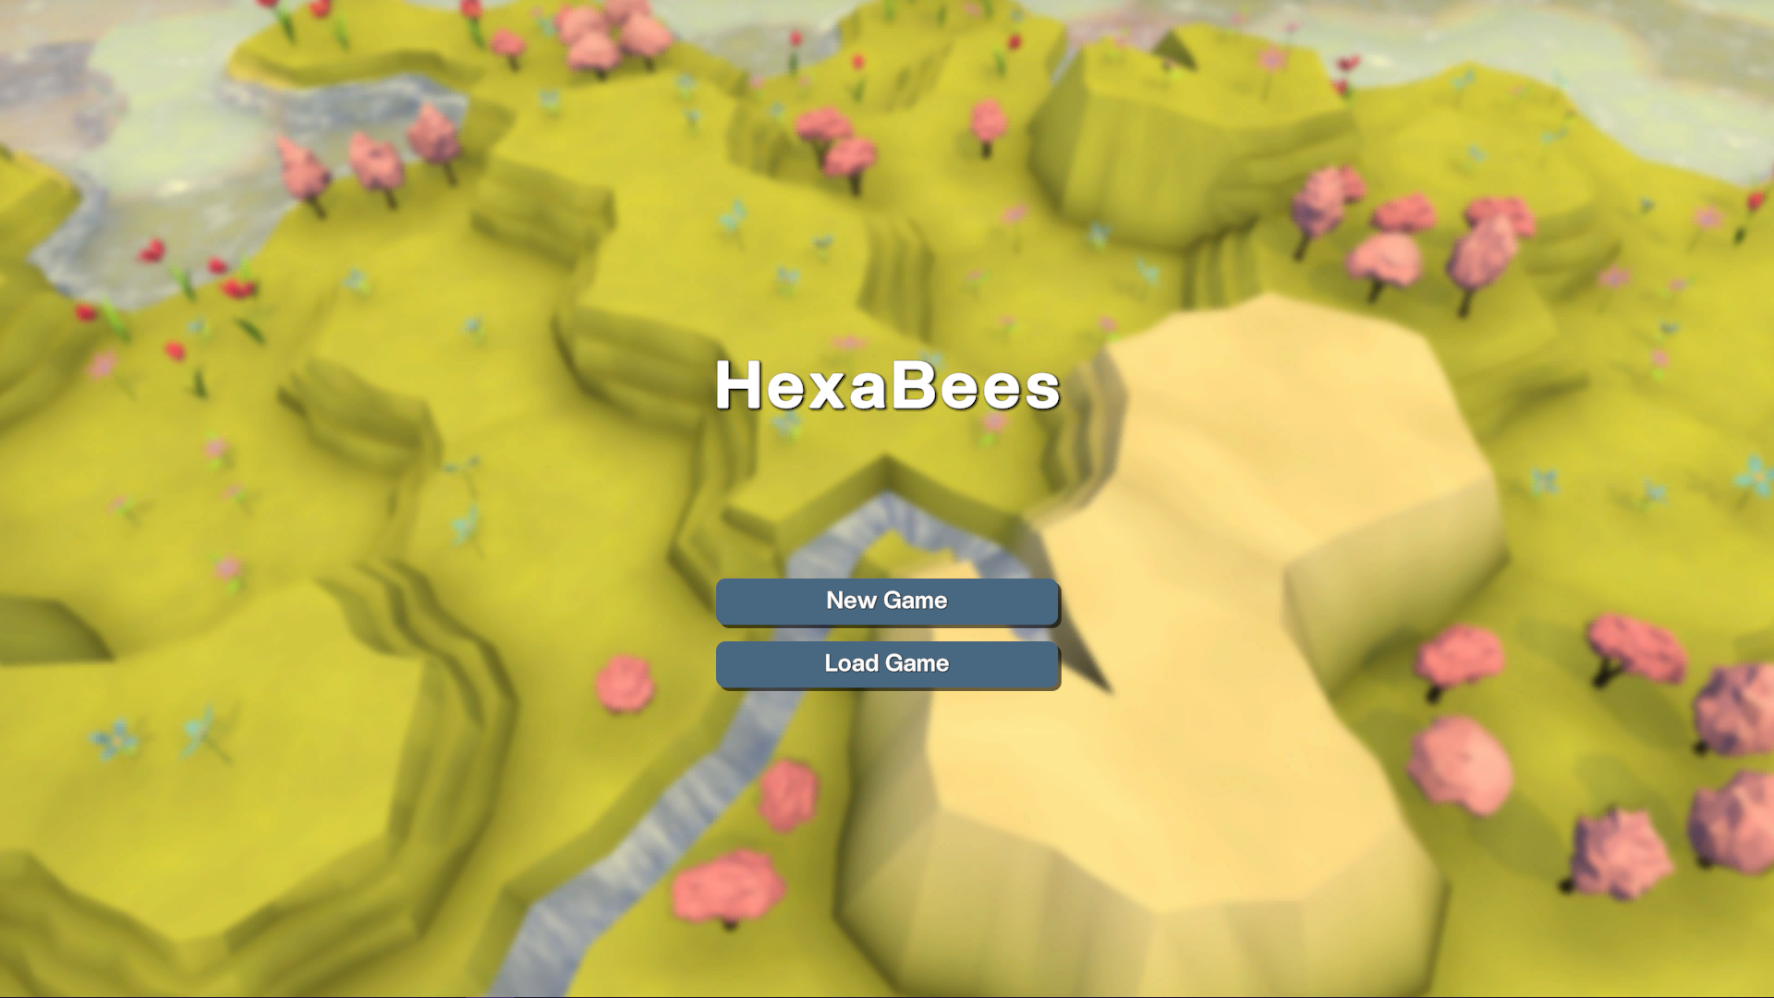
\includegraphics[width=300px]{0.bilder/startscreen.png}
    \end{center}
    \caption{Start Screen des Spiels} \label{image:startscreen}
\end{figure}